\documentclass[12pt,a4paper]{article}

\usepackage{amsfonts}
\usepackage{amsmath}
\usepackage{geometry}
\usepackage{graphicx}
\usepackage[dvipsnames,table]{xcolor}
\usepackage[subfolder,cleanup]{gnuplottex}
%\usepackage{amsthm}
%\usepackage{enumitem}
%\usepackage{wrapfig}
\usepackage{subcaption}
%\usepackage{hyperref}
\usepackage{tikz}

\usetikzlibrary{%
	decorations.pathreplacing,%
 	decorations.pathmorphing%
}

\pgfdeclaredecoration{simple line}{initial}{
  \state{initial}[width=\pgfdecoratedpathlength-1sp]{\pgfmoveto{\pgfpointorigin}}
  \state{final}{\pgflineto{\pgfpointorigin}}
}

\tikzset{
   oshift/.style={decorate,decoration={simple line,raise=#1}}
}

\rowcolors{2}{gray!10}{white}

\let\originalleft\left
\let\originalright\right
\renewcommand{\left}{\mathopen{}\mathclose\bgroup\originalleft}
\renewcommand{\right}{\aftergroup\egroup\originalright}

\newcommand{\diff}[3][]{\frac{d^{#1}#2}{d{#3}^{#1}}}
\newcommand{\pdiff}[3][]{\frac{\partial^{#1}#2}{\partial{#3}^{#1}}}

%\bibliographystyle{ieeetr}

\title{Position Sensing}
\author{Brady Metherall}
\date{October 28, 2019}

\newgeometry{margin=1in}
%\setlength\parindent{0pt}

\begin{document}
\maketitle

\section{Introduction}

\begin{figure}[htpb]
\centering
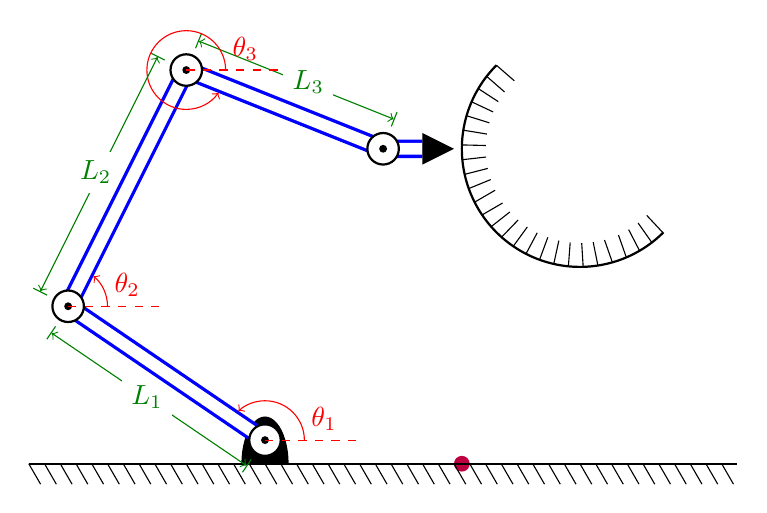
\begin{tikzpicture}
% Calibration point
\fill [purple] (2.5,0) circle (1mm);

% Ceiling
\draw [decorate,decoration={border,angle=-60,amplitude=3mm,segment length=2mm}] (-3,0) -- (6,0);
\draw [thick] (-3,0) -- (6,0);

% Car
\draw [decorate,decoration={border,angle=90,amplitude=3mm,segment length=1.88mm},domain=135:325] plot ({4+1.5*cos(\x)}, {4+1.5*sin(\x)});
\draw [thick,domain=135:315,samples=250] plot ({4+1.5*cos(\x)}, {4+1.5*sin(\x)});

% Anchor
\fill [domain=0:180] plot ({0.3*cos(\x)}, {0.6*sin(\x)});

% Lengths
\draw [|<->|,oshift=4mm,Green] (0,0.3) -- (-2.5,2) node [fill=white,pos=0.5,xshift=-2.5mm,yshift=-3mm] {$L_1$};
\draw [|<->|,oshift=4mm,Green] (-2.5,2) -- (-1,5) node [fill=white,pos=0.5,xshift=-4mm,yshift=2mm] {$L_2$};
\draw [|<->|,oshift=4mm,Green] (-1,5) -- (1.5,4) node [fill=white,pos=0.5,xshift=3mm,yshift=3.5mm] {$L_3$};

% Arms
\draw [blue,very thick,double,double distance=1.5mm] (0,0.3) -- (-2.5,2) -- (-1,5) -- (1.5,4) -- (2,4);
\fill (2,3.8) -- (2,4.2) -- (2.4,4) -- cycle;

% Joints
\draw [thick,fill=white] (0,0.3) circle (0.2);
\draw [thick,fill=white] (-2.5,2) circle (0.2);
\draw [thick,fill=white] (-1,5) circle (0.2);
\draw [thick,fill=white] (1.5,4) circle (0.2);
\fill (0,0.3) circle (0.05);
\fill (-2.5,2) circle (0.05);
\fill (-1,5) circle (0.05);
\fill (1.5,4) circle (0.05);

% Angles
\draw [red,dashed] (0,0.3) -- (1.25,0.3) node [pos=0.6,anchor=south] {$\theta_1$};
\draw [red,dashed] (-2.5,2) -- (-1.25,2) node [pos=0.6,anchor=south] {$\theta_2$};
\draw [red,dashed] (-1,5) -- (0.25,5) node [pos=0.6,anchor=south] {$\theta_3$};
\draw [->,red] (0.5,0.3) arc (0:132.5:0.5);
\draw [->,red] (-2,2) arc (0:50:0.5);
\draw [->,red] (-0.5,5) arc (0:325:0.5);

\end{tikzpicture}
\caption{}
\label{fig:scheme}
\end{figure}

\begin{figure}[htbp]
\centering
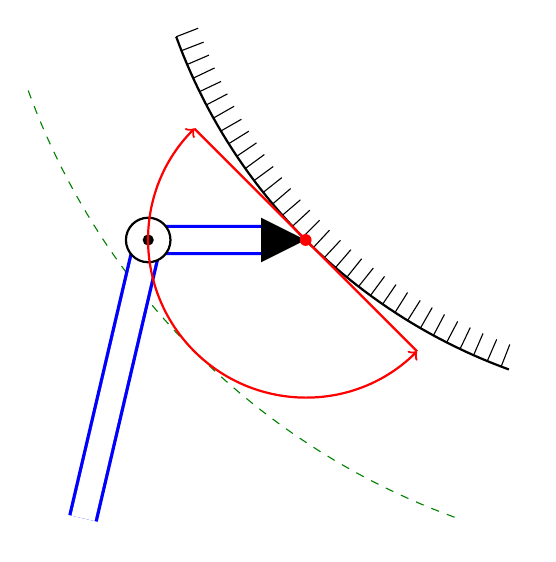
\begin{tikzpicture}[x=0.707cm,y=0.707cm]
% Car
\draw [decorate,decoration={border,angle=90,amplitude=3mm,segment length=1.895mm},domain=200:252] plot ({10/sqrt(2) + 10*cos(\x)}, {10/sqrt(2) + 10*sin(\x)});
\draw [thick,domain=200:250,samples=250] plot ({10/sqrt(2) + 10*cos(\x)}, {10/sqrt(2) + 10*sin(\x)});

% Green outline
\draw [domain=200:250,samples=250,Green,dashed] plot ({10/sqrt(2) + 12.82842*cos(\x)}, {10/sqrt(2) + 12.82842*sin(\x)});

% Arms
\draw [blue,very thick,double,double distance=3mm] (-4,-5) -- (-2.82842,0) -- (-0.7,0);
\fill (-0.8,-0.4) -- (-0.8,0.4) -- (0,0) -- cycle;

% Joint
\draw [thick,fill=white] (-2.82842,0) circle (0.4);
\fill (-2.82842,0) circle (0.1);

% Red semicircle
\fill [red] (0,0) circle (0.75mm); % Dot
\draw [thick,red] (-2,2) -- (2,-2); % Line
\draw [thick,red,<->] (-2,2) arc (135:315:2.82842); % Arc
\end{tikzpicture}
\caption{}
\label{fig:angle}
\end{figure}

\section{Model}

\subsection{Assumptions}

-rods are rigid and 0 width

-first hinge is on ceiling at 0,0

nd



$\theta$ is current position / state

$\varphi = \theta - \delta$ is initial position / state

\begin{align}
x &= \sum_{i=1}^N L_i \cos \theta_i; & y &= \sum_{i=1}^N L_i \sin \theta_i
\end{align}


\subsection{Calibration}

Known position
\begin{align}
1 &= \sum_{i=1}^N L_i \cos \varphi_i; & 0 &= \sum_{i=1}^N L_i \sin \varphi_i
\end{align}

second position
\begin{align}
1 &= \sum_{i=1}^N L_i \cos \left( \varphi_i + \delta_i \right); & 0 &= \sum_{i=1}^N L_i \sin \left( \varphi_i + \delta_i \right)
\end{align}

gives system of 4 eqns and 4 unknowns -> unique solution (up to modulus)



\section{Results}


\begin{table}[tbp]
\centering
\begin{tabular}{cccc}
Error 1 & Error 2 & Error 3 & Error 4 \\
\noalign{\global\arrayrulewidth=1.25pt}\hline
-0.07420 & \ 0.07420 & -0.04497 & -0.00179 \\
-0.07420 & \ 0.02742 & \ 0.02853 & -0.07487 \\
-0.02412 & -0.16026 & \ 0.27843 & -0.27794 \\
\ 0.07272 & \ 1.20678 & \ 4.78410 & \ 1.30220 \\
-0.71895 & \ 0.71895 & -0.52670 & -0.15747 \\
\hline
\end{tabular}
\caption{Sample data.}
\label{tab:data}
\end{table}

\begin{figure}[htbp]
\centering
\begin{gnuplot}[terminal=epslatex, terminaloptions={color size 6in,3.7in lw 3}]
#load '/home/brady/Templates/Blues.p'
set grid
set size ratio -1
set xl '$x$'
set yl rotate by 0 '$y$'
set xtics 0.5
set ytics 0.4
plot 'Shape.dat' u 1:2 dt 5 w l t 'Calibration', \
'Shape.dat' u 3:4 w l t 'Set 1', \
'Shape.dat' u 5:6 w l t 'Set 2', \
'Shape.dat' u 7:8 w l t 'Set 3'
\end{gnuplot}
\caption{}
\label{fig:}
\end{figure}

\begin{align*}
x_\text{err} = \frac{1}{2} \left| \sum_{i=1}^N L_i \left( \cos \left( \theta_i + \sum_{j=1}^i \phi_j^\text{tol} \right) - \cos \left( \theta_i - \sum_{j=1}^i \phi_j^\text{tol} \right) \right) \right|
\end{align*}

trig identities

simplify

note $\phi << 1$

\begin{align*}
x_\text{err} = \left| \sum_{i=1}^N L_i \sin \theta_i \sum_{j=1}^i \phi_j^\text{tol} \right|
\end{align*}

\begin{align*}
y_\text{err} = \left| \sum_{i=1}^N L_i \cos \theta_i \sum_{j=1}^i \phi_j^\text{tol} \right|
\end{align*}

\begin{align*}
\pdiff{x_\text{err}}{L_k} = \left| \sin \theta_k \sum_{j=1}^k \phi_j^\text{tol} \right|
\end{align*}

\begin{align*}
\pdiff{x_\text{err}}{\phi_k^\text{tol}} = \left| \sum_{i=k}^N L_i \sin \theta_i \right|
\end{align*}

\begin{figure}[htbp]
\centering
\begin{subfigure}{0.5\textwidth}
\begin{gnuplot}[terminal=epslatex, terminaloptions={color size 3.2in,3.2in lw 3}]
load './PlotStyle.p'
p 'Total.dat' u 1:2 pt 7 ps .5 lc rgb 'web-green' t 'Reachable', \
'Bottom6.dat' u 1:2 pt 7 ps 0.5 lc rgb 'red' t 'Unreachable', \
sqrt(0.6**2 - (x-1)**2) dt 5 t 'Minimum Reach'
\end{gnuplot}
\caption{}
\label{fig:}
\end{subfigure}%
\begin{subfigure}{0.5\textwidth}
\begin{gnuplot}[terminal=epslatex, terminaloptions={color size 3.2in,3.2in lw 3}]
#load '/home/brady/Templates/Blues.p'
load './PlotStyle.p'
p 'Total.dat' u 1:2 pt 7 ps .5 lc rgb 'web-green' t 'Reachable', \
'Top6.dat' u 1:2 pt 7 ps 0.5 lc rgb 'red' t 'Unreachable'
\end{gnuplot}
\caption{}
\label{fig:}
\end{subfigure}
\caption{$L_1 = 1$, $L_2 = 0.6$}
\label{fig:}
\end{figure}

\begin{figure}[htbp]
\centering
\begin{subfigure}{0.5\textwidth}
\begin{gnuplot}[terminal=epslatex, terminaloptions={color size 3.2in,3.2in lw 3}]
load './PlotStyle.p'
p 'Total.dat' u 1:2 pt 7 ps .5 lc rgb 'web-green' t 'Reachable', \
'Bottom4.dat' u 1:2 pt 7 ps 0.5 lc rgb 'red' t 'Unreachable', \
sqrt(1.475**2 - x**2) dt 5 t 'Maximum Reach'
\end{gnuplot}
\caption{}
\label{fig:}
\end{subfigure}%
\begin{subfigure}{0.5\textwidth}
\begin{gnuplot}[terminal=epslatex, terminaloptions={color size 3.2in,3.2in lw 3}]
load './PlotStyle.p'
p 'Total.dat' u 1:2 pt 7 ps .5 lc rgb 'web-green' t 'Reachable', \
'Top4.dat' u 1:2 pt 7 ps 0.5 lc rgb 'red' t 'Unreachable', \
sqrt(1.475**2 - x**2) dt 5 t 'Maximum Reach'
\end{gnuplot}
\caption{}
\label{fig:}
\end{subfigure}
\caption{$L_1 = 1$, $L_2 = 0.475$}
\label{fig:}
\end{figure}
\section{Conclusion}

\appendix
\section{Geometric Constraint}

\begin{align*}
t &= \frac{\sin \left(\theta _2\right)+\cos \left(\theta _2\right)-L_1 \cos \left(\theta _1-\theta _2\right)\pm\sqrt{\Delta}}{L_2} \\
\Delta &= -L_1^2 \sin ^2\left(\theta _1-\theta _2\right)+2 L_1 \sin \left(\theta _1-\theta _2\right) \left(\cos \left(\theta _2\right)-\sin \left(\theta _2\right)\right)+\sin \left(2 \theta _2\right)+R^2-1
\end{align*}


%\bibliography{Ref}

\end{document}




